%----------------------------------------------------------------------------------------
%	PACKAGES AND OTHER DOCUMENT CONFIGURATIONS
%----------------------------------------------------------------------------------------

\documentclass[
	letterpaper, % Page size
	fontsize=10pt, % Base font size
	twoside=true, % Use different layouts for even and odd pages 
                      % (in particular, if twoside=true, the margin column will be always on the outside)
	%open=any, % If twoside=true, uncomment this to force new chapters to start on any page, not only on right (odd) pages
	%chapterentrydots=true, % Uncomment to output dots from the chapter name to the page number in the table of contents
	numbers=noenddot, % Comment to output dots after chapter numbers; the most common values for this 
                          % option are: enddot, noenddot and auto (see the KOMAScript documentation for an in-depth explanation)
]{kaobook}

% Choose the language
\ifxetexorluatex
	\usepackage{polyglossia}
	\setmainlanguage{english}
\else
	\usepackage[english]{babel} % Load characters and hyphenation
\fi
\usepackage[english=british]{csquotes}	% English quotes

% Load packages for testing
\usepackage{blindtext} % Similar to lorem ipsum
%\usepackage{showframe} % Uncomment to show boxes around the text area, margin, header and footer
%\usepackage{showlabels} % Uncomment to output the content of \label commands to the document where they are used

% Load the bibliography package
\usepackage{kaobiblio}
\addbibresource{main.bib} % Bibliography file

% Load mathematical packages for theorems and related environments
\usepackage[framed=true]{kaotheorems}

% Load the package for hyperreferences
\usepackage{kaorefs}

\graphicspath{{examples/documentation/images/}{images/}} % Paths in which to look for images

\makeindex[columns=3, title=Alphabetical Index, intoc] % Make LaTeX produce the files required to compile the index

\makeglossaries % Make LaTeX produce the files required to compile the glossary
newglossaryentry{dictionaryEntry}{
    name={dictionary entry},
    description={is a set of data describing a Forth word}
}

\newglossaryentry{dictionary}{
    name={dictionary},
    description={dictionary description}
}

\newglossaryentry{nameField}{
    name={name field},
    description={name field description}
}

\newglossaryentry{linkField}{
    name={link field},
    description={link field description}
}

\newglossaryentry{parameterField}{
    name={parameter field},
    description={the address of a word's parameter field. The PFA points to the parameter field.}
}

\newglossaryentry{dataField}{
    name={data field},
    description={data see parameterField}
}

\newglossaryentry{codeField}{
    name={code field},
    description={code field description}
}

\newglossaryentry{linkFieldAddress}{
    name={link field address},
    description={link field address description}
}

\newglossaryentry{nameFieldAddress}{
    name={name field address},
    description={name field address description}
}

\newglossaryentry{parameterFieldAddress}{
    name={parameter field address},
    description={parameter field address description}
}

\newglossaryentry{codePointer}{
    name={code pointer},
    description={The address of the code. Stored in a word's code field. The Code Field Address is the addresss of the code field, not the address contained within the code field.}
}

\newglossaryentry{colonWord}{
    name={colon word},
    description={Colon-defined words have parameter fields that contain pointers to code fields in other words. These pointers are Code Field Addresses.}
}

\newglossaryentry{immediateWord}{
	name={immediate word},
	description={A word that has the IMMEDIATE bit set in its dictionary
    header. Is executed during interpretation. Is executed during 
    compilation rather than compiled into a definition. Is executed during compilation and interpretation}
}

\newglossaryentry{machine-code word}{
    name={Machine-code word},
    description={A word that is directly executed by the CPU. Does not 
    call other Forth words. May exit via a jump instruction to the 
    address of NEXT or by including the contents of NEXT inline, thereby 
    avoiding a jump instruction. Examples include the words NEXT EXECUTE 
    BRANCH and EXIT .}
}

\newglossaryentry{threadedCodeWord}{
    name={threaded- word},
    description={A word that contains other Forth words. May also contain machine-code words. Exits by calling the Forth word ; .}
}

\newglossaryentry{compileWord}{
        name={compile word},
        description={description}
}

% Glossary entries (used in text with e.g. \acrfull{fpsLabel} or \acrshort{fpsLabel})
\newacronym[longplural={Central Processor Units}]{cpuLabel}{CPU}{Central Processor Unit}
 % Include the glossary definitions

\makenomenclature % Make LaTeX produce the files required to compile the nomenclature

% Reset sidenote counter at chapters
%\counterwithin*{sidenote}{chapter}

% Load the package for byte field graphic generation
\usepackage{bytefield}
%---------------------------------------------------------------------------------------

\begin{document}

%----------------------------------------------------------------------------------------
%	BOOK INFORMATION
%----------------------------------------------------------------------------------------

%\titlehead{The \texttt{kaobook} class}
%\subject{Use this document as a template}

\title[The Forth Enlightenment]{The Forth Enlightenment}
\subtitle{Hardware for the Forth programming language}

\author[Charles Edward Pax]{Charles Edward Pax}

\date{\today}

\publishers{Self-publishing}

%----------------------------------------------------------------------------------------

\frontmatter % Denotes the start of the pre-document content, uses roman numerals

%----------------------------------------------------------------------------------------
%	OPENING PAGE
%----------------------------------------------------------------------------------------

%\makeatletter
%\extratitle{
%	% In the title page, the title is vspaced by 9.5\baselineskip
%	\vspace*{9\baselineskip}
%	\vspace*{\parskip}
%	\begin{center}
%		% In the title page, \huge is set after the komafont for title
%		\usekomafont{title}\huge\@title
%	\end{center}
%}
%\makeatother

%----------------------------------------------------------------------------------------
%	COPYRIGHT PAGE
%----------------------------------------------------------------------------------------

%\makeatletter
%\uppertitleback{\@titlehead} % Header
%
%\lowertitleback{
%	\textbf{Disclaimer}\\
%	Warranty disclaimer here
%	
%	\medskip
%	
%	\textbf{Copyright}\\
%	Copyright \textcopyright 2023 Charles Edward Pax. All rights reserved, for now.
%	
%	\medskip
%	
%	\textbf{Colophon} \\
%	This document was typeset with the help of \href{https://sourceforge.net/projects/koma-script/}{\KOMAScript} 
%       and \href{https://www.latex-project.org/}{\LaTeX} using the \href{https://github.com/fmarotta/kaobook/}{kaobook} class.
%	
%	The source code of this book template is available at:\\\url{https://github.com/fmarotta/kaobook}
%	
%	\medskip
%	
%	\textbf{Publisher} \\
%	First printed in December 2023 by \@publishers
%}
%\makeatother

%----------------------------------------------------------------------------------------
%	DEDICATION
%----------------------------------------------------------------------------------------

%\dedication{
%	It would be nice to have a dedication to a person or group of people.\\
%	\flushright -- Charles Edward Pax
%}

%----------------------------------------------------------------------------------------
%	OUTPUT TITLE PAGE AND PREVIOUS
%----------------------------------------------------------------------------------------

% Note that \maketitle outputs the pages before here

\maketitle

%----------------------------------------------------------------------------------------
%	PREFACE
%----------------------------------------------------------------------------------------

%\chapter*{Preface}
\addcontentsline{toc}{chapter}{Preface} % Add the preface to the table of contents as a chapter

This is the preface page. This book is broken into two parts:

\begin{itemize}
	\item Hardware
	\item Software
\end{itemize}

The main goal of this project is to create a system that a user can visually verify down
to the transistor level. The physical layout of the circuit should correspond to the
schematic drawing layout where possible.

\begin{flushright}
	\textit{Charles Edward Pax}
\end{flushright}

%\index{preface}

%----------------------------------------------------------------------------------------
%	TABLE OF CONTENTS & LIST OF FIGURES/TABLES
%----------------------------------------------------------------------------------------

\begingroup % Local scope for the following commands

% Define the style for the TOC, LOF, and LOT
%\setstretch{1} % Uncomment to modify line spacing in the ToC
%\hypersetup{linkcolor=blue} % Uncomment to set the colour of links in the ToC
\setlength{\textheight}{230\hscale} % Manually adjust the height of the ToC pages

% Turn on compatibility mode for the etoc package
\etocstandarddisplaystyle % "toc display" as if etoc was not loaded
\etocstandardlines % "toc lines" as if etoc was not loaded

\tableofcontents % Output the table of contents

%\listoffigures % Output the list of figures

% Comment both of the following lines to have the LOF and the LOT on different pages
\let\cleardoublepage\bigskip
\let\clearpage\bigskip

%\listoftables % Output the list of tables

\endgroup


%%%==============================================================================%%%
%%%==============================================================================%%%
%%%                                                                              %%%
%%%    ███╗   ███╗ █████╗ ██╗███╗   ██╗    ██████╗  ██████╗ ██████╗ ██╗   ██╗    %%%
%%%    ████╗ ████║██╔══██╗██║████╗  ██║    ██╔══██╗██╔═══██╗██╔══██╗╚██╗ ██╔╝    %%%
%%%    ██╔████╔██║███████║██║██╔██╗ ██║    ██████╔╝██║   ██║██║  ██║ ╚████╔╝     %%%
%%%    ██║╚██╔╝██║██╔══██║██║██║╚██╗██║    ██╔══██╗██║   ██║██║  ██║  ╚██╔╝      %%%
%%%    ██║ ╚═╝ ██║██║  ██║██║██║ ╚████║    ██████╔╝╚██████╔╝██████╔╝   ██║       %%%
%%%    ╚═╝     ╚═╝╚═╝  ╚═╝╚═╝╚═╝  ╚═══╝    ╚═════╝  ╚═════╝ ╚═════╝    ╚═╝       %%%
%%%                                                                              %%%
%%%  https://patorjk.com/software/taag/#p=display&f=ANSI%20Shadow&t=MAIN%20BODY  %%%
%%%==============================================================================%%%
%%%==============================================================================%%%

\mainmatter % Denotes the start of the main document content, resets page numbering and uses arabic numbers
\setchapterstyle{kao} % Choose the default chapter heading style

\setchapterimage{seaside}
\setchapterpreamble[u]{\margintoc}
\chapter{Introduction}
\labch{intro}

%
% Key concepts and abilities
%==============================================================================
\begin{kaobox}[frametitle=In This Chapter]
you will learn
\begin{itemize}
	\item First topic
	\item Second topic
        \item Third topic
\end{itemize}

you will be able to
\begin{itemize}
        \item Task one
        \item Task two
        \item Task three
\end{itemize}
\end{kaobox}

% Introductory paragraph goes here
\blindtext

%
% Section: Purpose %
%==============================================================================
\section{Purpose}
\labsec{purpose}

The purpose of this book is to address the necessity of trustless 
computing or verifyable computing.

\begin{itemize}
	\item Don't trust, verify
	\item trustless computing
	\item trusting the compiler
\end{itemize}

Design princples: simplicity is a virtue.

%=================================%
% Subsection: Don't trust, verify %
%=================================%
\subsection*{Don't trust, verify}
In this section talk about blah blah blah.

%=================================%
% Subsection: Trustless computing %
%=================================%
\subsection*{Trustless computing}
Discuss trustless computing here.

%===================================%
% Subsection: Trusting the compiler %
%===================================%
\subsection*{Trusting the compilers}
In this subsection there will be a discussion of trusting the compiler.

%==================================%
% Subsection: Application: Bitcoin %
%==================================%
\subsection*{Application: Bitcoin}
These topics are relevant to Bitcoin because it relates to money. Don't
get hacket. Artificial Intelligence is coming for your money.


%
% Section: Hardware Overview %
%==============================================================================
\section{Hardware Overview}
\labsec{hardwareOverview}

No microcode. Implement logic in hardware. Complex optimization is bad. conceptual
simplicity. Simplicity is a cirtue.

\begin{description}
	\item[visual verification] view with your own eyes
	\item[simplicity] keep it simple to understand
        \item[repitation] repeat blocks
\end{description}

\subsection*{Stack computers}
\begin{itemize}
        \item Why stack computers?
        \item Parts of a stack computer
        \item Types of stack computers
\end{itemize}

Do we cover the instruction cycle here? Instruction timing?

%
% Section: Instruction Set Architecture %
%==============================================================================
\section{Instruction set Architecture}
\labsec{isa}
\index{instruction set architecture}

The instruction set architecture should be kept simple. Each bit encodes specific information.

%
% Section: Software Overview %
%==============================================================================
\labsec{softwareOverview}

The software should:

\begin{itemize}
	\item be simple
        \item reuse code blocks
        \item not require a compiler
        \item be hand-writable
\end{itemize}

Threaded code. No compiler. Forth.

\setchapterimage{seaside}
\setchapterpreamble[u]{\margintoc}
\chapter{Hardware}
\labch{hardware}

%
% Key concepts and abilities
%==============================================================================
\begin{kaobox}[frametitle=In This Chapter]
you will learn
\begin{itemize}
	\item First topic
	\item Second topic
        \item Third topic
\end{itemize}

you will be able to
\begin{itemize}
        \item Task one
        \item Task two
        \item Task three
\end{itemize}
\end{kaobox}

% Introductory paragraph goes here
\blindtext

%
% Section: Stack Computers
%==============================================================================
\section{Stack Computers}
We will discuss stack computers\sidecite{Koopman1989}.


\setchapterimage{seaside}
\setchapterpreamble[u]{\margintoc}
\chapter{Instruction Set Architecture (ISA)}
\labch{isa}

%
% Key concepts and abilities
%==============================================================================
\begin{kaobox}[frametitle=In This Chapter]
you will learn
\begin{itemize}
	\item First topic
	\item Second topic
        \item Third topic
\end{itemize}

you will be able to
\begin{itemize}
        \item Task one
        \item Task two
        \item Task three
\end{itemize}
\end{kaobox}

% Introductory paragraph goes here
\blindtext

%
% Section: ISA Explained
%==============================================================================
\section{ISA Explained}
Explain what an ISA is.

%
% Section: Instruction cycle
%==============================================================================
\section{Instruction cycle}
\blindtext

\begin{figure}[hbt!]
\begin{bytefield}[bitwidth=auto]{16}
    \bitheader[endianness=big]{15,14,0} \\
\begin{rightwordgroup}{name field}
    \begin{leftwordgroup}[leftcurly=.]{address ($a$)}
        \bitbox{1}{$p$} &
        \bitbox{15}{$n$}
    \end{leftwordgroup} \\
    \bitbox{16}{$name_0$} \\
    \wordbox[]{1}{$\vdots$} \\[1ex]
    \begin{leftwordgroup}[leftcurly=.]{$a$ + $n$}
        \bitbox{16}{$name_n$}
    \end{leftwordgroup}
\end{rightwordgroup} \\
\begin{rightwordgroup}[rightcurly=.]{link address field}
    \begin{leftwordgroup}[leftcurly=.]{$a$ + $n$ + 1}
        \wordbox{1}{link address}
    \end{leftwordgroup}
\end{rightwordgroup} \\
\begin{rightwordgroup}[rightcurly=.]{code address field}
    \begin{leftwordgroup}[leftcurly=.]{$a$ + $n$ + 2}
        \wordbox{1}{code address}
    \end{leftwordgroup}
\end{rightwordgroup} \\
\begin{rightwordgroup}{data field ($d \ge 1$ cell)}
    \begin{leftwordgroup}[leftcurly=.]{$a$ + $n$ + 3}
        \wordbox{1}{$data_0$}
    \end{leftwordgroup} \\
    \wordbox[]{1}{$\vdots$} \\[1ex]
    \begin{leftwordgroup}[leftcurly=.]{$a$ + $n + 3 + d$}
    \wordbox{1}{$data_d$}
    \end{leftwordgroup}
\end{rightwordgroup}
\end{bytefield}

\caption[Dictionary entry format]{This is the MacroController Forth dictionary 
    entry format for a 16-bit system. Other Forth systems may implement a differnt format.}
	\labfig{dictionaryEntryFormat}
\end{figure}

where \\
$a$ is the address of the word, \\
$p$ is the precedence bit (0,1), \\
$n$ is the number of characters in the word's name (e.g. DUP$_n = 3$), \\
$name_n$ is the $n^{th}$ character of the name, \\
$d$ is the number of cells in the data field, and \\
$data_d$ is the $d^{th}$ cell of the data field.

%
% Section: Instruction Format
%==============================================================================
\section{Instruction Format}

%
% Section: Instruction Timing
%==============================================================================
\section{Instruction Timing}
\blindtext

\begin{figure}[hbt!]
\begin{tikztimingtable}
    Clock & 3{10{c}} \\
    Name & 3{hLLLLh} \\
    Signal & 3{z4D{Text}z} \\
\end{tikztimingtable}
\caption[Timing diagram]{This is an example timing diagram that will be replaced by the real thing.}
\end{figure}

\begin{figure}[hbt!]
\begin{tikzpicture}[
    myline/.style={draw=green!40!black, thick},
    box/.style={myline, minimum height=1cm, minimum width=1cm, font=\sffamily, inner sep=.3333em}, >=Stealth]

    \matrix (CPU) [matrix of nodes, inner ysep=3mm, nodes=box, myline, column sep=1mm]
        {|(CU)|CU & |[draw=none]|CPU & |(ALU)| ALU \\};
    \node[box, above left=5mm of CPU] (input) {INPUT};

    \node[box, below left=5mm of CPU] (output) {OUTPUT};
    \node[box, at=(CPU|-output)] (memory) {MEMORY};
    \node[box, below left=5mm of memory, anchor=north] (storage) {STORAGE};

    \draw[<->, myline] (storage)-|(memory);
    \draw[->,myline] (input)-|(CU);
    \draw[->,myline] (CU)|-(output);

    \draw[<->, myline] ($(CU.south west)!.2!(CU.south east)$) coordinate (aux)--(aux|-storage.north);
    \draw[<->, myline] ($(CU.south west)!.8!(CU.south east)$) coordinate (aux)--(aux|-memory.north);
    \draw[<->, myline] ($(ALU.south west)!.2!(ALU.south east)$) coordinate (aux)--(aux|-memory.north);
\end{tikzpicture}\caption[Timing diagram]{This is an example timing diagram that will be replaced by the real thing.}
\end{figure}


































\setchapterimage{seaside}
\setchapterpreamble[u]{\margintoc}
\chapter{The Forth Programming Language}
\labch{forth}

%
% Key concepts and abilities
%==============================================================================
\begin{kaobox}[frametitle=In This Chapter]
you will learn
\begin{itemize}
	\item First topic
	\item Second topic
        \item Third topic
\end{itemize}

you will be able to
\begin{itemize}
        \item Task one
        \item Task two
        \item Task three
\end{itemize}
\end{kaobox}

% Introductory paragraph goes here
\blindtext

%
% Section: Dictionay Entry Format
%====================================================================
\section{Dictionary Entry Format}

Each word in Forth is defined by a \gls{dictionaryEntry}
\gls{immediateWord}.



The dictionary entry format is dependent upon the Forth implmentation, but a typical
16-bit Forth system will implement the structure described in \reffig{dictionaryEntryFormat}.


\todo{Add headings for these three columns: Address, Contents, Description}
\begin{figure}[hbt!]
\begin{bytefield}[bitwidth=auto]{16}
    \begin{rightwordgroup}[rightcurly=.]{\textbf{Notes}}
            \begin{leftwordgroup}[leftcurly=.]{\textbf{Address}}
                \wordbox[]{1}{\textbf{Content}}
    \end{leftwordgroup}
\end{rightwordgroup} \\
    \bitheader[endianness=big]{15,14,0} \\
\begin{rightwordgroup}{name field}
    \begin{leftwordgroup}[leftcurly=.]{Name Field Address (NFA)}
        \bitbox{1}{$p$} &
        \bitbox{15}{$n$}
    \end{leftwordgroup} \\
    \begin{leftwordgroup}[leftcurly=.]{NFA $+ 1$}
        \bitbox{16}{$name_0$}
    \end{leftwordgroup} \\
    \wordbox[]{1}{$\vdots$} \\[1ex]
    \begin{leftwordgroup}[leftcurly=.]{NFA $+ n + 1$}
        \bitbox{16}{$name_n$}
    \end{leftwordgroup}
\end{rightwordgroup} \\
\begin{rightwordgroup}[rightcurly=.]{link field}
    \begin{leftwordgroup}[leftcurly=.]{Link Field Address (LFA)}
        \wordbox{1}{link pointer}
    \end{leftwordgroup}
\end{rightwordgroup} \\
\begin{rightwordgroup}[rightcurly=.]{code field}
    \begin{leftwordgroup}[leftcurly=.]{Code Field Addresss (CFA)}
        \wordbox{1}{code pointer}
    \end{leftwordgroup}
\end{rightwordgroup} \\
\begin{rightwordgroup}{parameter field}
    \begin{leftwordgroup}[leftcurly=.]{Parameter Field Address (PFA)}
        \wordbox{1}{$parameter_0$}
    \end{leftwordgroup} \\
    \wordbox[]{1}{$\vdots$} \\[1ex]
    \begin{leftwordgroup}[leftcurly=.]{PFA $+ c$}
    \wordbox{1}{$parameter_c$}
    \end{leftwordgroup}
\end{rightwordgroup}
\end{bytefield}

\caption[Dictionary entry format]{Dictionary entry format.}
	\labfig{dictionaryEntryFormat}
\end{figure}

where \\
\todo{how are these items sorted? Alphabetical? Order of appearance?}
NFA is the address pointing to the first cell in the word's name field, \\
LFA is the address pointing to the word's link pointer field, \\
CFA is the address pointing to the word's code pointer field, \\
PFA is the address pointing to the first cell in the word's parameter field, \\
$p$ is the precedence bit (0,1), \\
$n$ is the number of characters in the word's name (e.g. DUP$_n = 3$), \\
$name_n$ is the $n^{th}$ character in the name, \\
$c$ is the number of cells in the parameter field, and \\
$parameter_c$ is the $c^{th}$ cell in the parameter field.

Each dictionary entry has a link pointer field, which holds an memory address pointing to the 
preceeding dictionary entry. By design, when the system searches for a word it starts 
at the end of the dictionary and works its way to the beginning by following these 
pointers. We call these addresses link pointers because they link the words together and to
distinguish them from pointers with other purposes.




The link pointer of a dictionary entry points to the name field of the previous word. The value of a link pointer is equal to the NFA of the pervious dictionary entry.
The link pointer is an address pointing to the first cell of the previous dictionary entry's name field. The LFA of a dictionary entry contains the NFA of the previous dictionary entry.i

, \\
code address is the address of the machine instruction the interpreter will load for
execution, and \\
data is any data that is required for execution.

\todo[noline]{Decide if the name field characters are 16-bit or 8-bit in the final implementation.}
\marginnote{The code address field is also known as the code pointer field. The data field
is also known as the parameter field.}

Precedence bit. 0 - address of the word gets compiled normally. 1 - The word is executed 
during compilation.

Are the characters in the name field limited to ASCII? Is there any technical reason they
could not be any arbitrary 16-bit value? Maybe null would be a problem.

Leo Brodie's Starting Forth\sidecite{Brodie1981} is good reading for this.

%
% Section: The Forth Inner Interpreter
%====================================================================
\section{The Forth Inner Interpreter}
This section gives a general explaination\sidenote[]{Use sidenotes if necessary} 
of the chapter topic\sidecite{Loeliger1981}.

The word \lstinline|:| causes the innter interpreter to enter compile mode. The name of the
word is next, followed by the definition. The word \lstinline|;| causes the inner
interpreter to exit compilation and reenter interpretation mode.

Example:
\begin{lstlisting}[caption={Definition of \lstinline|dup| in Forth.}]
: square ( x -- x )
    dup
    *
    :
\end{lstlisting}

This, of course, can be more conveniently written on a single line
\begin{lstlisting}[style=kaolstplain,linewidth=1.5\textwidth]
: square ( x -- x )
    dup * ;
\end{lstlisting}

\section{Return Stack}
The top of the return stack holds the return address. When a function call is made, the return address
must be stored.  If the call command is executed at address x, the return address x+1 is pushed to the top of the return stack.

\section{Data Stack}
The data styack is where temporary data is stored.

If a system has only one hardware stack, it shoulld be used for the data stack. Data 
manipulations are more common than function calls and the hardware stack is faster 
than memory access. The call stack will need to be stored in memory.

For "colon words" (words compiled with the : word), the data field is a series of cells, each cell
containing an address pointing to a word in the Forth dictionary.

The address interpreter (inner interpreter) copies the address stored in the address field
into the interpreter pointer then executes the code at that address.

The interpreter does not keep track of or know about the type of word it is working with. The code linked to by the CFA is responsible for behaving appropriately.

%
% Section: The Forth Outter Interpreter
%====================================================================
\section{The Forth Outter Interpreter}
This an intermediate section. There will be several. each such section will cover a
discrete topic within this chapter.

\marginnote{Margin notes can be used to explain detail or add reminders that would
otherwise break the flow of the document. I think sidenotes are numbered while
margin notes are not.}

\blindtext

\setchapterimage{seaside}
\setchapterpreamble[u]{\margintoc}
\chapter{Template Chapter}
\labch{chaptertemplate}

%
% Key concepts and abilities
%==============================================================================
\begin{kaobox}[frametitle=In This Chapter]
you will learn
\begin{itemize}
	\item what is the first topic
	\item how to identify the second topic
        \item best practices for the third topic
\end{itemize}

you will be able to
\begin{itemize}
        \item perform the steps required to accomplish task one
        \item create a program that performs task two
\end{itemize}
\end{kaobox}

This introduction gives the reader any context necessary to understand the 
proceeding sections in this chapter.

The contents of the `In This Chapter' box should concrete. This should coorespond to
a `Chapter Review' section at the end of the chapter.

Illuminate any common obstacles for the reader. A few words of encouragement are also welcomed.

%
% Section: Heaps of Examples
%==============================================================================
\section{Heaps of Examples}
This section is fairly dense with examples. You can delete everything from here until
the end of the page.\sidenote[]{After you have saved this document as a new file.}

This section serves as an easy way to demonstrate\footnote{Like this footnote} multiple 
graphical elements\todo{Add a list of elements} that can be used in this book.

Keep chapters, sections, and sub sections capitalized.

%
% Subsection: Margin Stuff
%------------------------------------------------------------------------------
\subsection{Margin Stuff}
Generally, any text that would be written between parentheses would do well as
a margin note. Keep the flow going.

\marginnote{
	\begin{kaobox}[frametitle=Remember]
		a kaobox can be used in the margins for special reminders)
	\end{kaobox}
}

%
% Subsubsection: Sections in Depth
%
\subsubsection{Sections in Depth}
Sections within a chapter can be \Command{section}, \Command{subsection}, or
\Command{subsubsection}\marginnote{Notice that \Command{subsubsection} does not cause numbering.}.

%
% Subsection: Figures and Tables}
%------------------------------------------------------------------------------
\subsection{Figures and Tables}
\begin{lstlisting}[caption={
This Forth code does NOT generate \reftab{useless}
}]
: square  ( x -- x )
( Forth code that squares a number
    dup * ;
\end{lstlisting}

This is an example of a table contained withing the main column of text.

\begin{table}[ht]
\caption[A useless table]{A useless table.}
\labtab{useless}
\begin{tabular}{ c c c c }
    \toprule
    col1          & col2  & col3  & col4\\
    \midrule
    \multirow{3}{4em}{
    Multiple row} & 
        cell2 & cell3 & cell4\\ &
        cell5 & cell6 & cell7 \\ &
        cell8 & cell9 & cell10 \\
    \multirow{3}{4em}{
    Multiple row} & 
        cell2 & cell3 & cell4 \\ &
        cell5 & cell6 & cell7 \\ &
        cell8 & cell9 & cell10 \\
    \bottomrule
\end{tabular}
\end{table}


We can also have full-width tables.

\begin{table*}[h!]
    \caption{A wide table with invented data about three people living in the UK. Note that wide figures and tables are centered and their caption also extends into the margin.}
    \begin{tabular}{p{2.0cm} p{2.0cm} p{2.0cm} p{2.0cm} p{2.0cm} p{2.0cm} p{1.5cm}}
        \toprule
        Name    & Surname   & Job       & Salary           & Age   & Height    & Country \\
        \midrule
        Alice   & Red       & Writer    & 4.000 \pounds    & 34    & 167 cm     & England \\
        Bob     & White     & Bartender & 2.000 \pounds    & 24    & 180 cm     & Scotland \\
        Drake   & Green     & Scientist & 4.000 \pounds    & 26    & 175 cm     & Wales \\
        \bottomrule
    \end{tabular}
\end{table*}

And full-width images.

\blindtext

\begin{figure*}[h!]
	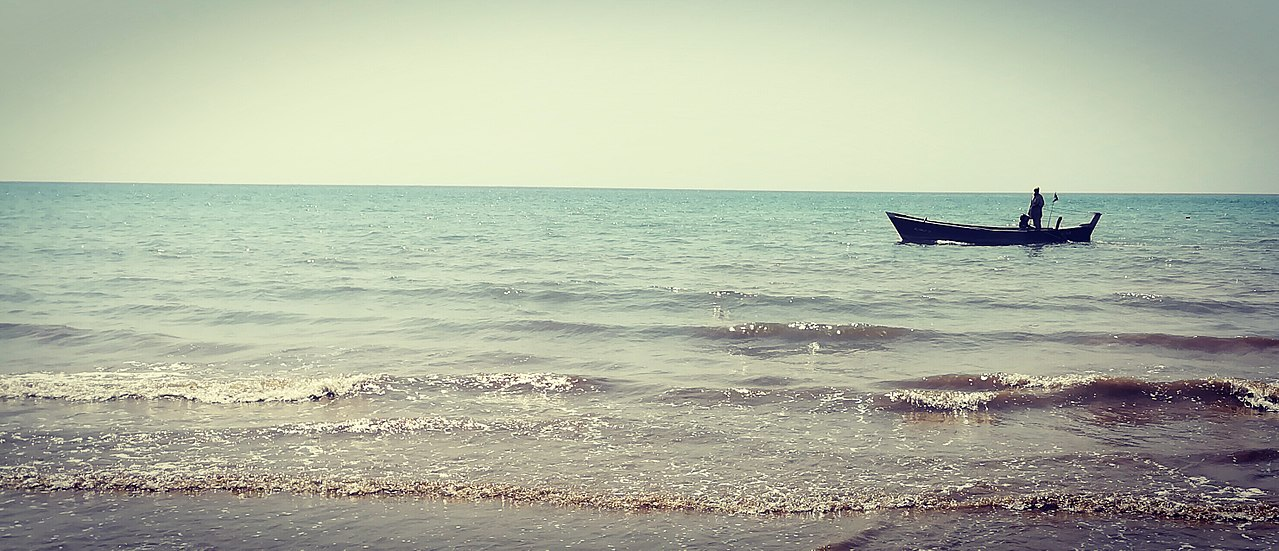
\includegraphics{seaside}
	\caption[A wide seaside]{A wide seaside, and a wide caption.
		Credits: By Bushra Feroz, CC BY-SA 4.0, \url{https://commons.wikimedia.org/w/index.php?curid=68724647}}
\end{figure*}

\begin{marginfigure}
	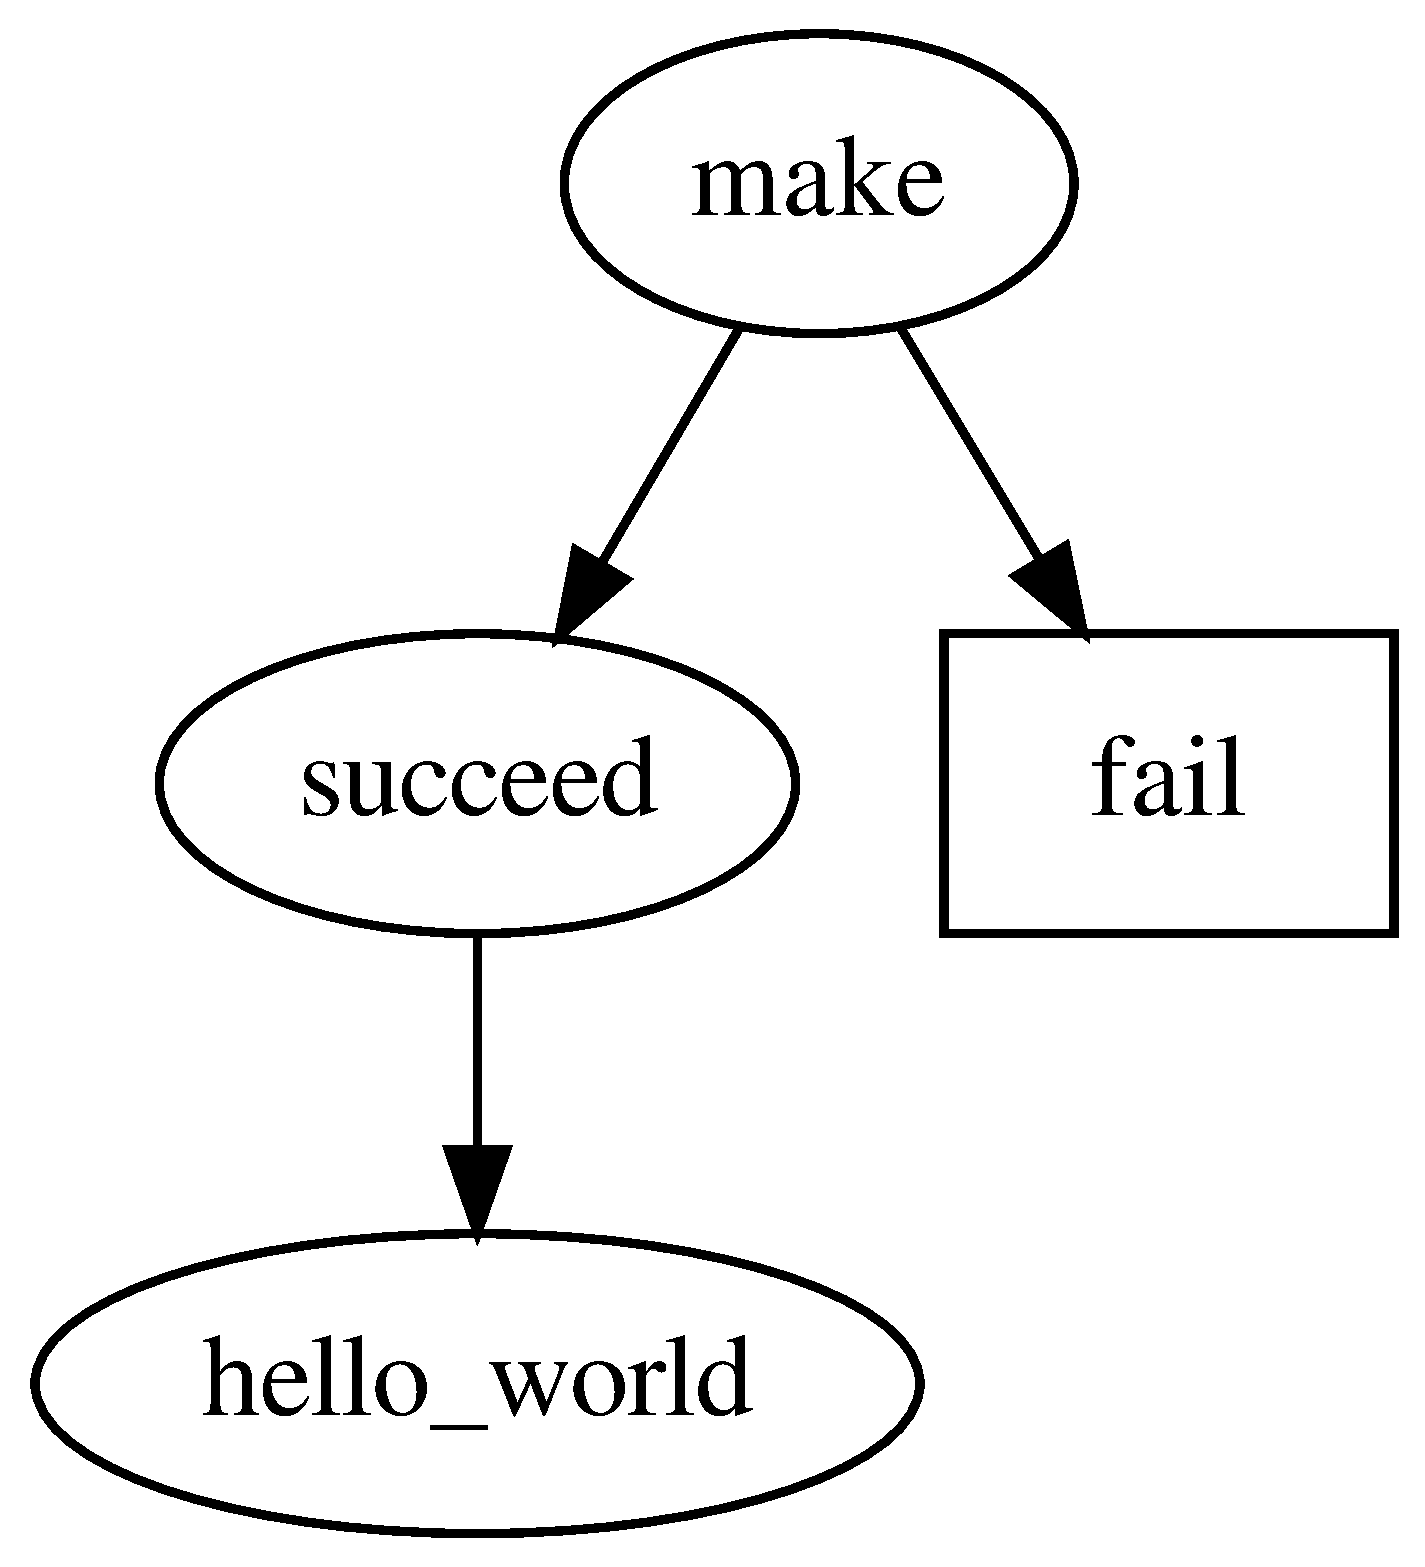
\includegraphics{output2}
	\caption[A Dot diagram]{A diagram produced by the Dot program and saved as a PNG file.}
	\labfig{marginmonalisa}
\end{marginfigure}

%
% Subsection: Citations
%------------------------------------------------------------------------------
\subsection{Citations}
Cite an author in the margin\sidecite{example1999}.

\blindtext


%
% Subsection: Glossaries and Indicies
%------------------------------------------------------------------------------
\subsection{Glossaries and Indicies}

%
% Subsection: Mathematics
%------------------------------------------------------------------------------
\subsection{Mathematics}
The box below was created using the \Environment{definition} environment. Boxes are also
provided by the \Environment{theorem}, \Environment{proposition}, \Environment{lemma},
\Environment{corollary}, \Environment{example}, \Environment{remark}, and \Environment{exercise} environments.

\begin{definition}
\labdef{exdeflabel}
Let $y$ be some function of $x$ such that $y = f(x)$
\end{definition}

where $x$ and $y$ are both variables in \refdef{exdeflabel}.



\blindtext

%
% Chapter Review
%==============================================================================
\section{Chapter Review}
\begin{kaobox}[frametitle=Chapter Review]
you have learned
\begin{itemize}
	\item what is the first topic
	\item how to identify the second topic
        \item best practices for the third topic
\end{itemize}

you are able to
\begin{itemize}
        \item perform the steps required to accomplish task one
        \item create a program that performs task two
\end{itemize}
\end{kaobox}








\appendix % From here onwards, chapters are numbered with letters, as is the appendix convention

\setchapterstyle{lines}
\labch{appendix}
%\blinddocument

\chapter{Template Appendix}

%
% Section: One section
%==============================================================================
\section{One section}

\blindtext


%
% Section: Another Section
%==============================================================================
\section{Another Section}

\blindtext


%----------------------------------------------------------------------------------------

\backmatter % Denotes the end of the main document content
\setchapterstyle{plain} % Output plain chapters from this point onwards

%----------------------------------------------------------------------------------------
%	BIBLIOGRAPHY
%----------------------------------------------------------------------------------------

% The bibliography needs to be compiled with biber using your LaTeX editor, or on the command line with 'biber main' from the template directory

\defbibnote{bibnote}{Works are listed in order of first citation.\par\bigskip} % Prepend this text to the bibliography
\printbibliography[heading=bibintoc, title=Bibliography, prenote=bibnote] % Add the bibliography heading to the ToC, set the title of the bibliography and output the bibliography note

%----------------------------------------------------------------------------------------
%	NOMENCLATURE
%----------------------------------------------------------------------------------------

% The nomenclature needs to be compiled on the command line with 'makeindex main.nlo -s nomencl.ist -o main.nls' from the template directory

\nomenclature{$c$}{Speed of light in a vacuum inertial frame}
\nomenclature{$h$}{Planck constant}

\renewcommand{\nomname}{Notation} % Rename the default 'Nomenclature'
\renewcommand{\nompreamble}{The next list describes several symbols that will be later used within the body of the document.} % Prepend this text to the nomenclature

%\printnomenclature % Output the nomenclature

%----------------------------------------------------------------------------------------
%	GLOSSARY
%----------------------------------------------------------------------------------------

% The glossary needs to be compiled on the command line with 'makeglossaries main' from the template directory

\setglossarystyle{altlist} % Set the style of the glossary (see https://en.wikibooks.org/wiki/LaTeX/Glossary for a reference)
\glsaddall % print all terms in the glossary, not only referenced words
\printglossary[title=Glossary, toctitle=Glossary,nonumberlist] % Output the glossary, 'title' is the chapter heading for the glossary, toctitle is the table of contents heading

%----------------------------------------------------------------------------------------
%	INDEX
%----------------------------------------------------------------------------------------

% The index needs to be compiled on the command line with 'makeindex main' from the template directory

%\printindex % Output the index

%----------------------------------------------------------------------------------------
%	BACK COVER
%----------------------------------------------------------------------------------------

% If you have a PDF/image file that you want to use as a back cover, uncomment the following lines

%\clearpage
%\thispagestyle{empty}
%\null%
%\clearpage
%\includepdf{cover-back.pdf}

%----------------------------------------------------------------------------------------

\end{document}
